% GNUPLOT: LaTeX picture with Postscript
\begingroup
  \makeatletter
  \providecommand\color[2][]{%
    \GenericError{(gnuplot) \space\space\space\@spaces}{%
      Package color not loaded in conjunction with
      terminal option `colourtext'%
    }{See the gnuplot documentation for explanation.%
    }{Either use 'blacktext' in gnuplot or load the package
      color.sty in LaTeX.}%
    \renewcommand\color[2][]{}%
  }%
  \providecommand\includegraphics[2][]{%
    \GenericError{(gnuplot) \space\space\space\@spaces}{%
      Package graphicx or graphics not loaded%
    }{See the gnuplot documentation for explanation.%
    }{The gnuplot epslatex terminal needs graphicx.sty or graphics.sty.}%
    \renewcommand\includegraphics[2][]{}%
  }%
  \providecommand\rotatebox[2]{#2}%
  \@ifundefined{ifGPcolor}{%
    \newif\ifGPcolor
    \GPcolorfalse
  }{}%
  \@ifundefined{ifGPblacktext}{%
    \newif\ifGPblacktext
    \GPblacktexttrue
  }{}%
  % define a \g@addto@macro without @ in the name:
  \let\gplgaddtomacro\g@addto@macro
  % define empty templates for all commands taking text:
  \gdef\gplbacktext{}%
  \gdef\gplfronttext{}%
  \makeatother
  \ifGPblacktext
    % no textcolor at all
    \def\colorrgb#1{}%
    \def\colorgray#1{}%
  \else
    % gray or color?
    \ifGPcolor
      \def\colorrgb#1{\color[rgb]{#1}}%
      \def\colorgray#1{\color[gray]{#1}}%
      \expandafter\def\csname LTw\endcsname{\color{white}}%
      \expandafter\def\csname LTb\endcsname{\color{black}}%
      \expandafter\def\csname LTa\endcsname{\color{black}}%
      \expandafter\def\csname LT0\endcsname{\color[rgb]{1,0,0}}%
      \expandafter\def\csname LT1\endcsname{\color[rgb]{0,1,0}}%
      \expandafter\def\csname LT2\endcsname{\color[rgb]{0,0,1}}%
      \expandafter\def\csname LT3\endcsname{\color[rgb]{1,0,1}}%
      \expandafter\def\csname LT4\endcsname{\color[rgb]{0,1,1}}%
      \expandafter\def\csname LT5\endcsname{\color[rgb]{1,1,0}}%
      \expandafter\def\csname LT6\endcsname{\color[rgb]{0,0,0}}%
      \expandafter\def\csname LT7\endcsname{\color[rgb]{1,0.3,0}}%
      \expandafter\def\csname LT8\endcsname{\color[rgb]{0.5,0.5,0.5}}%
    \else
      % gray
      \def\colorrgb#1{\color{black}}%
      \def\colorgray#1{\color[gray]{#1}}%
      \expandafter\def\csname LTw\endcsname{\color{white}}%
      \expandafter\def\csname LTb\endcsname{\color{black}}%
      \expandafter\def\csname LTa\endcsname{\color{black}}%
      \expandafter\def\csname LT0\endcsname{\color{black}}%
      \expandafter\def\csname LT1\endcsname{\color{black}}%
      \expandafter\def\csname LT2\endcsname{\color{black}}%
      \expandafter\def\csname LT3\endcsname{\color{black}}%
      \expandafter\def\csname LT4\endcsname{\color{black}}%
      \expandafter\def\csname LT5\endcsname{\color{black}}%
      \expandafter\def\csname LT6\endcsname{\color{black}}%
      \expandafter\def\csname LT7\endcsname{\color{black}}%
      \expandafter\def\csname LT8\endcsname{\color{black}}%
    \fi
  \fi
    \setlength{\unitlength}{0.0500bp}%
    \ifx\gptboxheight\undefined%
      \newlength{\gptboxheight}%
      \newlength{\gptboxwidth}%
      \newsavebox{\gptboxtext}%
    \fi%
    \setlength{\fboxrule}{0.5pt}%
    \setlength{\fboxsep}{1pt}%
\begin{picture}(5760.00,4032.00)%
    \gplgaddtomacro\gplbacktext{%
      \csname LTb\endcsname%%
      \put(4667,-65){\makebox(0,0)[l]{\strut{}$R$ (\AA)}}%
      \put(77,2294){\rotatebox{90}{\makebox(0,0)[l]{\strut{}$u_{IS-SPA}$ (kcal/mol)}}}%
      \put(30,440){\makebox(0,0)[l]{\strut{}\color{white}.}}%
    }%
    \gplgaddtomacro\gplfronttext{%
      \csname LTb\endcsname%%
      \put(4508,1712){\makebox(0,0)[r]{\strut{}CDD + LJ}}%
      \csname LTb\endcsname%%
      \put(4508,1492){\makebox(0,0)[r]{\strut{}$|q|=1$ e -- explicit}}%
      \csname LTb\endcsname%%
      \put(4508,1272){\makebox(0,0)[r]{\strut{}$q=0$ e -- explicit}}%
      \csname LTb\endcsname%%
      \put(4508,1052){\makebox(0,0)[r]{\strut{}$q=+1$ e -- IS-SPA}}%
      \csname LTb\endcsname%%
      \put(4508,832){\makebox(0,0)[r]{\strut{}$q=-1$ e -- IS-SPA}}%
      \csname LTb\endcsname%%
      \put(4508,612){\makebox(0,0)[r]{\strut{}$q=0$ e -- IS-SPA}}%
      \csname LTb\endcsname%%
      \put(594,440){\makebox(0,0)[r]{\strut{}$-35$}}%
      \csname LTb\endcsname%%
      \put(594,861){\makebox(0,0)[r]{\strut{}$-30$}}%
      \csname LTb\endcsname%%
      \put(594,1283){\makebox(0,0)[r]{\strut{}$-25$}}%
      \csname LTb\endcsname%%
      \put(594,1704){\makebox(0,0)[r]{\strut{}$-20$}}%
      \csname LTb\endcsname%%
      \put(594,2126){\makebox(0,0)[r]{\strut{}$-15$}}%
      \csname LTb\endcsname%%
      \put(594,2547){\makebox(0,0)[r]{\strut{}$-10$}}%
      \csname LTb\endcsname%%
      \put(594,2968){\makebox(0,0)[r]{\strut{}$-5$}}%
      \csname LTb\endcsname%%
      \put(594,3390){\makebox(0,0)[r]{\strut{}$0$}}%
      \csname LTb\endcsname%%
      \put(594,3811){\makebox(0,0)[r]{\strut{}$5$}}%
      \csname LTb\endcsname%%
      \put(726,220){\makebox(0,0){\strut{}$0$}}%
      \csname LTb\endcsname%%
      \put(1035,220){\makebox(0,0){\strut{}$1$}}%
      \csname LTb\endcsname%%
      \put(1344,220){\makebox(0,0){\strut{}$2$}}%
      \csname LTb\endcsname%%
      \put(1653,220){\makebox(0,0){\strut{}$3$}}%
      \csname LTb\endcsname%%
      \put(1963,220){\makebox(0,0){\strut{}$4$}}%
      \csname LTb\endcsname%%
      \put(2272,220){\makebox(0,0){\strut{}$5$}}%
      \csname LTb\endcsname%%
      \put(2581,220){\makebox(0,0){\strut{}$6$}}%
      \csname LTb\endcsname%%
      \put(2890,220){\makebox(0,0){\strut{}$7$}}%
      \csname LTb\endcsname%%
      \put(3199,220){\makebox(0,0){\strut{}$8$}}%
      \csname LTb\endcsname%%
      \put(3508,220){\makebox(0,0){\strut{}$9$}}%
      \csname LTb\endcsname%%
      \put(3817,220){\makebox(0,0){\strut{}$10$}}%
      \csname LTb\endcsname%%
      \put(4126,220){\makebox(0,0){\strut{}$11$}}%
      \csname LTb\endcsname%%
      \put(4436,220){\makebox(0,0){\strut{}$12$}}%
      \csname LTb\endcsname%%
      \put(4745,220){\makebox(0,0){\strut{}$13$}}%
      \csname LTb\endcsname%%
      \put(5054,220){\makebox(0,0){\strut{}$14$}}%
      \csname LTb\endcsname%%
      \put(5363,220){\makebox(0,0){\strut{}$15$}}%
      \csname LTb\endcsname%%
      \put(958,3592){\makebox(0,0){\strut{}\Large{(a)}}}%
    }%
    \gplgaddtomacro\gplbacktext{%
      \csname LTb\endcsname%%
      \put(10263,-65){\makebox(0,0)[l]{\strut{}$R$ (\AA)}}%
      \put(5733,2126){\rotatebox{90}{\makebox(0,0)[l]{\strut{}$\delta u_{IS-SPA}^{LJ}$ (kcal/mol)}}}%
      \put(5495,440){\makebox(0,0)[l]{\strut{}\color{white}.}}%
    }%
    \gplgaddtomacro\gplfronttext{%
      \csname LTb\endcsname%%
      \put(10123,3634){\makebox(0,0)[r]{\strut{}LJ}}%
      \csname LTb\endcsname%%
      \put(10123,3414){\makebox(0,0)[r]{\strut{}$q=+1$ e -- explicit}}%
      \csname LTb\endcsname%%
      \put(10123,3194){\makebox(0,0)[r]{\strut{}$q=-1$ e -- explicit}}%
      \csname LTb\endcsname%%
      \put(10123,2974){\makebox(0,0)[r]{\strut{}$|q|=0$ e -- explicit LJ}}%
      \csname LTb\endcsname%%
      \put(10123,2754){\makebox(0,0)[r]{\strut{}$q=+1$ e -- IS-SPA}}%
      \csname LTb\endcsname%%
      \put(10123,2534){\makebox(0,0)[r]{\strut{}$q=-1$ e -- IS-SPA}}%
      \csname LTb\endcsname%%
      \put(10123,2314){\makebox(0,0)[r]{\strut{}$q=0$ e -- IS-SPA}}%
      \csname LTb\endcsname%%
      \put(6078,440){\makebox(0,0)[r]{\strut{}$-4$}}%
      \csname LTb\endcsname%%
      \put(6078,1002){\makebox(0,0)[r]{\strut{}$-2$}}%
      \csname LTb\endcsname%%
      \put(6078,1564){\makebox(0,0)[r]{\strut{}$0$}}%
      \csname LTb\endcsname%%
      \put(6078,2126){\makebox(0,0)[r]{\strut{}$2$}}%
      \csname LTb\endcsname%%
      \put(6078,2687){\makebox(0,0)[r]{\strut{}$4$}}%
      \csname LTb\endcsname%%
      \put(6078,3249){\makebox(0,0)[r]{\strut{}$6$}}%
      \csname LTb\endcsname%%
      \put(6078,3811){\makebox(0,0)[r]{\strut{}$8$}}%
      \csname LTb\endcsname%%
      \put(6210,220){\makebox(0,0){\strut{}$0$}}%
      \csname LTb\endcsname%%
      \put(6528,220){\makebox(0,0){\strut{}$1$}}%
      \csname LTb\endcsname%%
      \put(6846,220){\makebox(0,0){\strut{}$2$}}%
      \csname LTb\endcsname%%
      \put(7164,220){\makebox(0,0){\strut{}$3$}}%
      \csname LTb\endcsname%%
      \put(7481,220){\makebox(0,0){\strut{}$4$}}%
      \csname LTb\endcsname%%
      \put(7799,220){\makebox(0,0){\strut{}$5$}}%
      \csname LTb\endcsname%%
      \put(8117,220){\makebox(0,0){\strut{}$6$}}%
      \csname LTb\endcsname%%
      \put(8435,220){\makebox(0,0){\strut{}$7$}}%
      \csname LTb\endcsname%%
      \put(8753,220){\makebox(0,0){\strut{}$8$}}%
      \csname LTb\endcsname%%
      \put(9071,220){\makebox(0,0){\strut{}$9$}}%
      \csname LTb\endcsname%%
      \put(9389,220){\makebox(0,0){\strut{}$10$}}%
      \csname LTb\endcsname%%
      \put(9707,220){\makebox(0,0){\strut{}$11$}}%
      \csname LTb\endcsname%%
      \put(10024,220){\makebox(0,0){\strut{}$12$}}%
      \csname LTb\endcsname%%
      \put(10342,220){\makebox(0,0){\strut{}$13$}}%
      \csname LTb\endcsname%%
      \put(10660,220){\makebox(0,0){\strut{}$14$}}%
      \csname LTb\endcsname%%
      \put(10978,220){\makebox(0,0){\strut{}$15$}}%
      \csname LTb\endcsname%%
      \put(6448,3592){\makebox(0,0){\strut{}\Large{(b)}}}%
    }%
    \gplgaddtomacro\gplbacktext{%
      \csname LTb\endcsname%%
      \put(15970,-65){\makebox(0,0)[l]{\strut{}$R$ (\AA)}}%
      \put(11381,2463){\rotatebox{90}{\makebox(0,0)[l]{\strut{}$\delta u_{pmf}^{C}$ (kcal/mol)}}}%
      \put(11335,440){\makebox(0,0)[l]{\strut{}\color{white}.}}%
    }%
    \gplgaddtomacro\gplfronttext{%
      \csname LTb\endcsname%%
      \put(15810,1510){\makebox(0,0)[r]{\strut{}CDD}}%
      \csname LTb\endcsname%%
      \put(15810,1290){\makebox(0,0)[r]{\strut{}$q=+1$ e -- explicit}}%
      \csname LTb\endcsname%%
      \put(15810,1070){\makebox(0,0)[r]{\strut{}$q=-1$ e -- explicit}}%
      \csname LTb\endcsname%%
      \put(15810,850){\makebox(0,0)[r]{\strut{}$q=+1$ e -- IS-SPA}}%
      \csname LTb\endcsname%%
      \put(15810,630){\makebox(0,0)[r]{\strut{}$q=-1$ e -- IS-SPA}}%
      \csname LTb\endcsname%%
      \put(11898,440){\makebox(0,0)[r]{\strut{}$-50$}}%
      \csname LTb\endcsname%%
      \put(11898,1114){\makebox(0,0)[r]{\strut{}$-40$}}%
      \csname LTb\endcsname%%
      \put(11898,1788){\makebox(0,0)[r]{\strut{}$-30$}}%
      \csname LTb\endcsname%%
      \put(11898,2463){\makebox(0,0)[r]{\strut{}$-20$}}%
      \csname LTb\endcsname%%
      \put(11898,3137){\makebox(0,0)[r]{\strut{}$-10$}}%
      \csname LTb\endcsname%%
      \put(11898,3811){\makebox(0,0)[r]{\strut{}$0$}}%
      \csname LTb\endcsname%%
      \put(12030,220){\makebox(0,0){\strut{}$0$}}%
      \csname LTb\endcsname%%
      \put(12339,220){\makebox(0,0){\strut{}$1$}}%
      \csname LTb\endcsname%%
      \put(12648,220){\makebox(0,0){\strut{}$2$}}%
      \csname LTb\endcsname%%
      \put(12957,220){\makebox(0,0){\strut{}$3$}}%
      \csname LTb\endcsname%%
      \put(13266,220){\makebox(0,0){\strut{}$4$}}%
      \csname LTb\endcsname%%
      \put(13575,220){\makebox(0,0){\strut{}$5$}}%
      \csname LTb\endcsname%%
      \put(13884,220){\makebox(0,0){\strut{}$6$}}%
      \csname LTb\endcsname%%
      \put(14193,220){\makebox(0,0){\strut{}$7$}}%
      \csname LTb\endcsname%%
      \put(14502,220){\makebox(0,0){\strut{}$8$}}%
      \csname LTb\endcsname%%
      \put(14811,220){\makebox(0,0){\strut{}$9$}}%
      \csname LTb\endcsname%%
      \put(15120,220){\makebox(0,0){\strut{}$10$}}%
      \csname LTb\endcsname%%
      \put(15429,220){\makebox(0,0){\strut{}$11$}}%
      \csname LTb\endcsname%%
      \put(15738,220){\makebox(0,0){\strut{}$12$}}%
      \csname LTb\endcsname%%
      \put(16047,220){\makebox(0,0){\strut{}$13$}}%
      \csname LTb\endcsname%%
      \put(16356,220){\makebox(0,0){\strut{}$14$}}%
      \csname LTb\endcsname%%
      \put(16665,220){\makebox(0,0){\strut{}$15$}}%
      \csname LTb\endcsname%%
      \put(12262,3592){\makebox(0,0){\strut{}\Large{(c)}}}%
    }%
    \gplbacktext
    \put(0,0){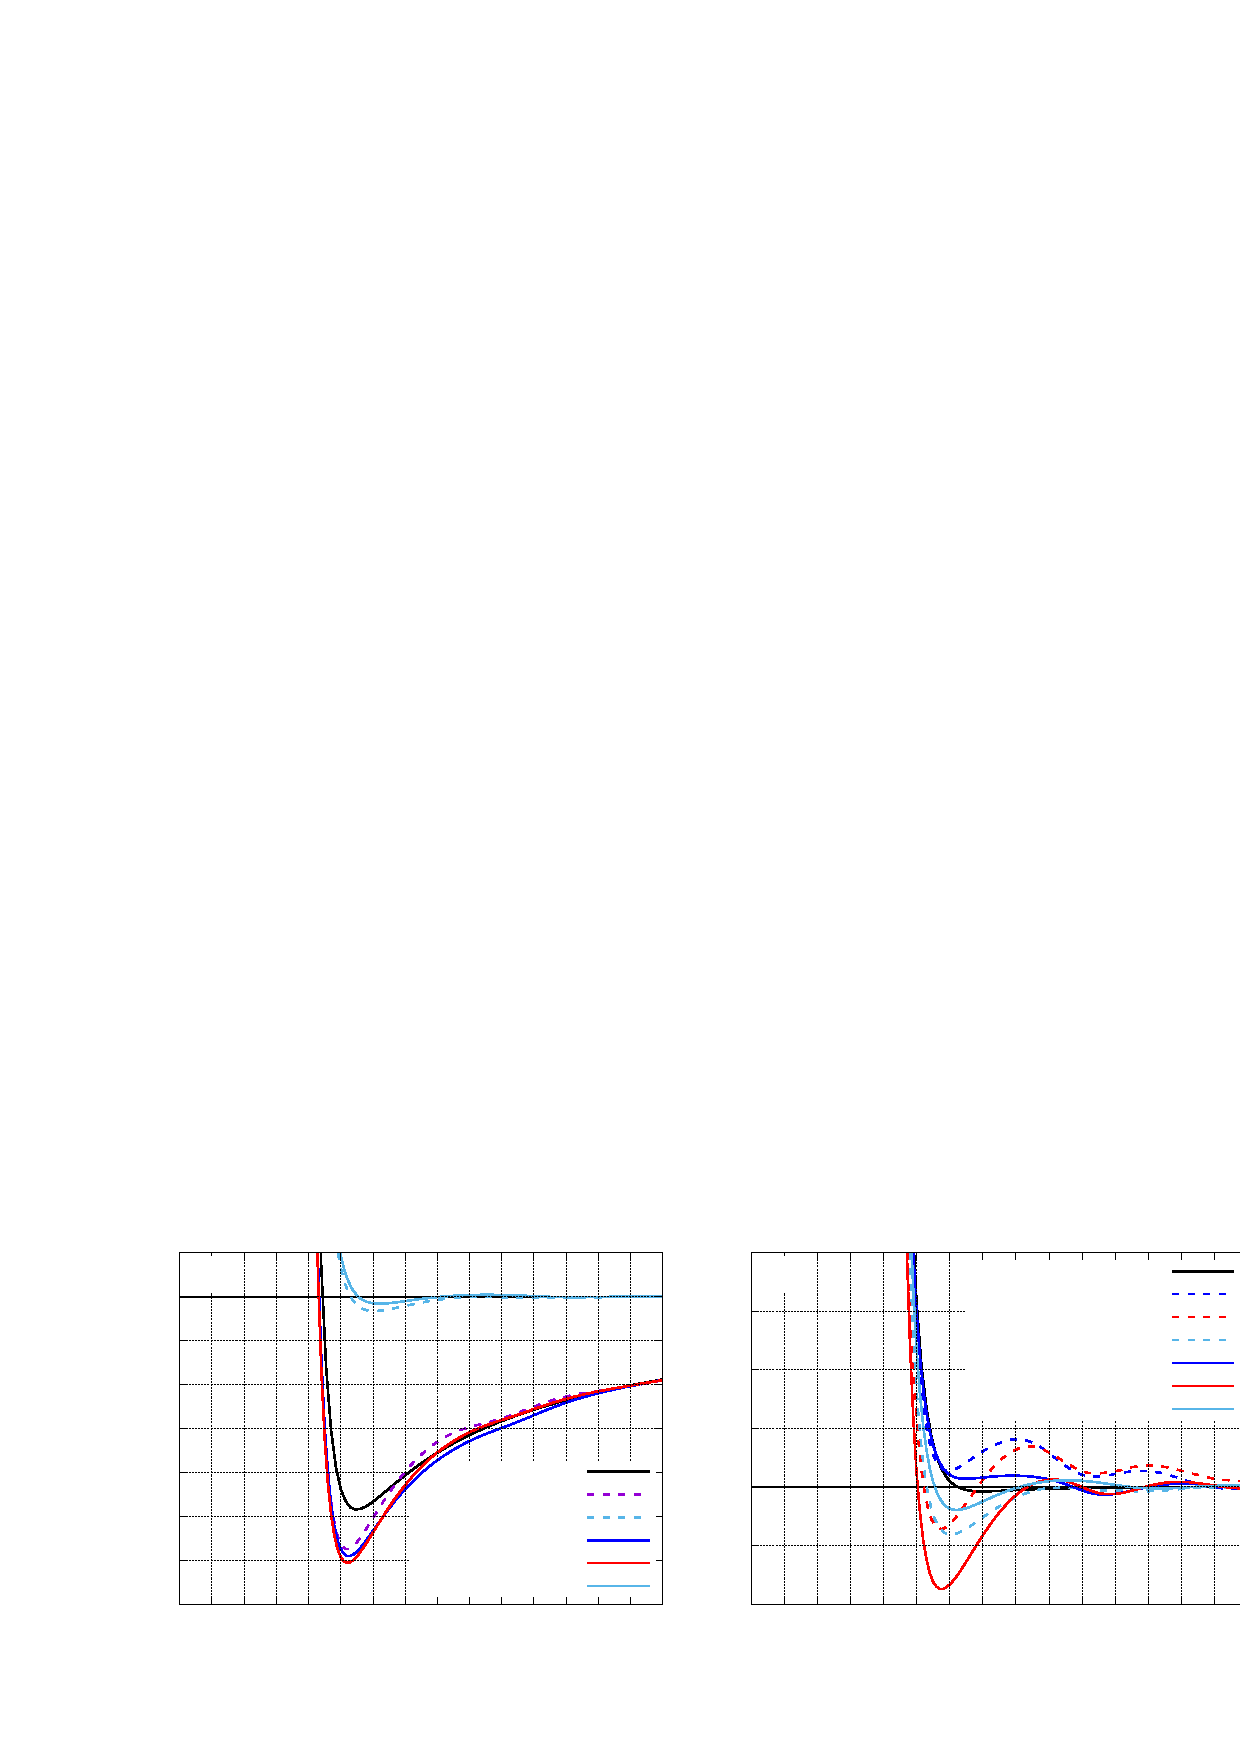
\includegraphics{test}}%
    \gplfronttext
  \end{picture}%
\endgroup
